% Ejemplo de BSG (w = 2, m = 4): dos niveles de la busqueda en haz, cada hijo evaluado con su
% completacion greedy; se conservan los w mejores y se devuelve la mejor solucion completa
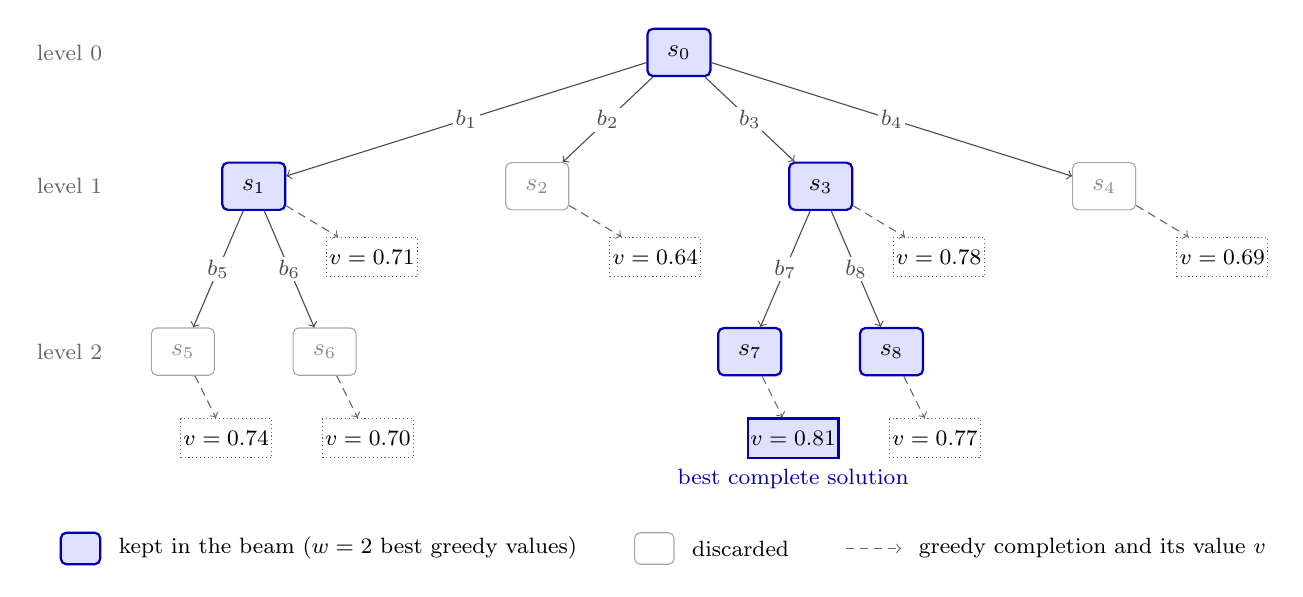
\begin{tikzpicture}[
	font=\small,
	st/.style={draw, rounded corners=2pt, minimum width=8mm, minimum height=6mm, inner sep=1pt},
	kept/.style={st, fill=blue!12, draw=blue!70!black, thick},
	pruned/.style={st, draw=black!35, text=black!45},
	leaf/.style={draw=black!60, densely dotted, minimum width=11mm, minimum height=5mm, inner sep=1pt, font=\footnotesize},
	best/.style={leaf, draw=blue!70!black, solid, thick, fill=blue!12},
	blk/.style={font=\footnotesize, inner sep=1pt, fill=white},
	gr/.style={->, densely dashed, black!60},
	lvl/.style={font=\footnotesize, text=black!60, anchor=east},
]
% nivel 0
\node[kept] (s0) at (0,0) {$s_0$};
% nivel 1: m = 4 hijos de la raiz
\foreach \i/\x/\v/\k in {1/-5.4/0.71/kept, 2/-1.8/0.64/pruned, 3/1.8/0.78/kept, 4/5.4/0.69/pruned}{
	\node[\k] (a\i) at (\x,-1.7) {$s_\i$};
	\draw[->, black!70] (s0) -- node[blk] {$b_\i$} (a\i);
	\node[leaf] (va\i) at (\x+1.5,-2.6) {$v = \v$};
	\draw[gr] (a\i) -- (va\i);
}
% nivel 2: cada nodo del haz se expande con m/w = 2 bloques
\foreach \p/\i/\x/\v/\k in {1/5/-6.3/0.74/pruned, 1/6/-4.5/0.70/pruned, 3/7/0.9/0.81/kept, 3/8/2.7/0.77/kept}{
	\node[\k] (b\i) at (\x,-3.8) {$s_\i$};
	\draw[->, black!70] (a\p) -- node[blk] {$b_\i$} (b\i);
}
\foreach \i/\x/\v/\s in {5/-6.3/0.74/leaf, 6/-4.5/0.70/leaf, 7/0.9/0.81/best, 8/2.7/0.77/leaf}{
	\node[\s] (vb\i) at (\x+0.55,-4.9) {$v = \v$};
	\draw[gr] (b\i) -- (vb\i);
}
\node[font=\footnotesize, text=blue!70!black, anchor=north] at (vb7.south) {best complete solution};
% niveles
\node[lvl] at (-7.2,0) {level 0};
\node[lvl] at (-7.2,-1.7) {level 1};
\node[lvl] at (-7.2,-3.8) {level 2};
% leyenda
\begin{scope}[shift={(-7.6,-6.3)}]
	\node[kept, minimum width=5mm, minimum height=4mm] (l1) at (0,0) {};
	\node[anchor=west, font=\footnotesize] (t1) at (l1.east) {\ kept in the beam ($w = 2$ best greedy values)};
	\node[pruned, minimum width=5mm, minimum height=4mm, anchor=west] (l2) at ([xshift=6mm]t1.east) {};
	\node[anchor=west, font=\footnotesize] (t2) at (l2.east) {\ discarded};
	\draw[gr] ([xshift=6mm]t2.east) -- ++(0.7,0) coordinate (l3);
	\node[anchor=west, font=\footnotesize] at (l3) {\ greedy completion and its value $v$};
\end{scope}
\end{tikzpicture}
